\documentclass{article}
\usepackage[utf8]{inputenc}
\usepackage{algorithm}
\usepackage{algpseudocode}
\usepackage{graphicx}
\usepackage{amsmath,amssymb,amsthm, ,amsfonts}

\title{Location Prediction Algorithm}
\author{Shashank Sharma }
\date{August 2018}

\begin{document}

\maketitle

\section{Introduction}
This algorithm is designed to predict human locations in a real world scenario. The GPS data is taken as input and the processed using the below algorithm.


The Algorithm has several steps:
\begin{itemize}
\item Detect stay-points (also detect start or end of the trajectory)
\item Group stay-points to form states
\item Calculate hourly weights for the states
\item Apply Markov chain for the data available
\end{itemize}

\begin{figure}[h!]
\centering
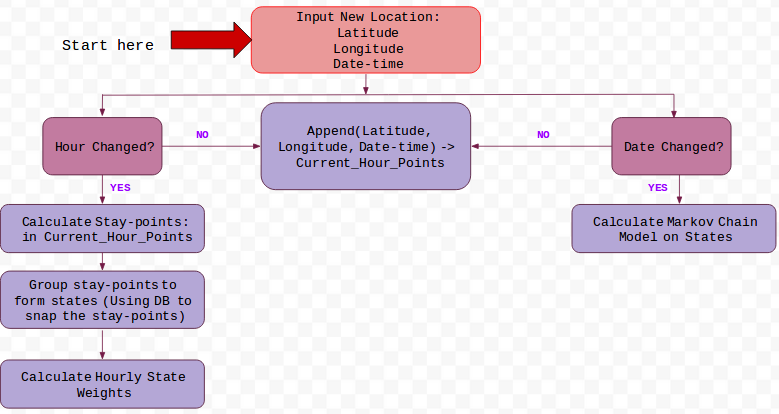
\includegraphics[scale=.46]{Flowchart_Algo.png}
\caption{Algorithm Flow-chart}
\label{fig:flow-chart}
\end{figure}

\begin{figure}[h!]
\centering
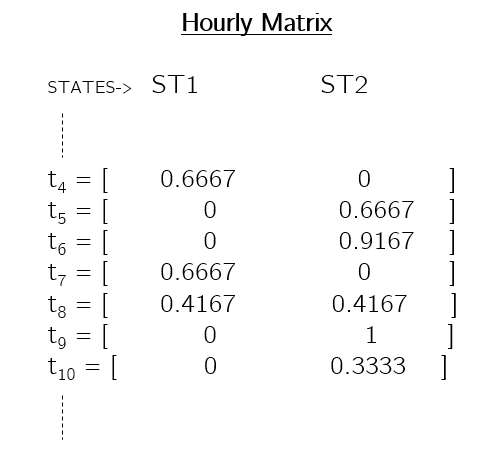
\includegraphics[scale=.34]{hourlymat.png}
\caption{Algorithm Flow-chart}
\label{fig:flow-chart}
\end{figure}

\begin{figure}[h!]
\centering
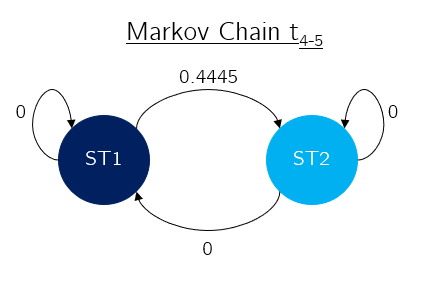
\includegraphics[scale=.35]{markovchain.png}
\caption{Algorithm Flow-chart}
\label{fig:flow-chart}
\end{figure}

\begin{figure}[h!]
\centering
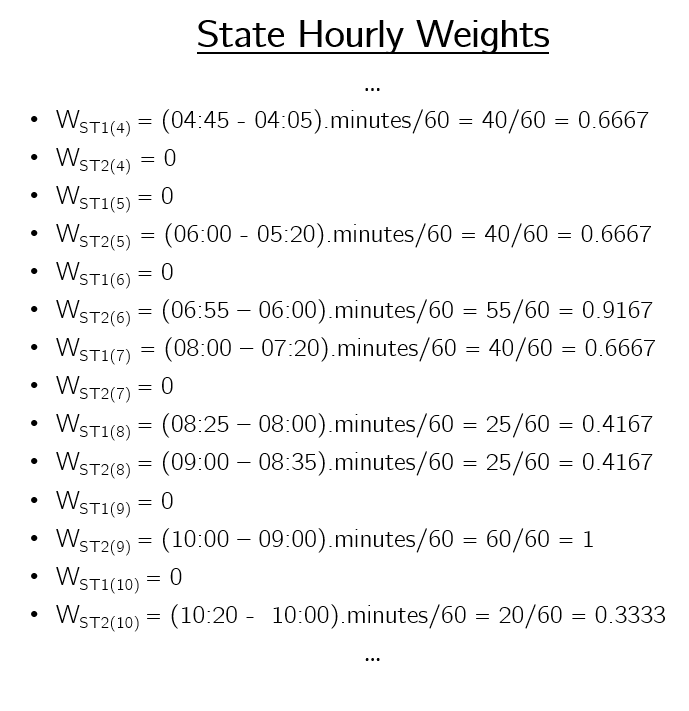
\includegraphics[scale=.35]{stateweights.png}
\caption{Algorithm Flow-chart}
\label{fig:flow-chart}
\end{figure}

\begin{figure}[h!]
\centering
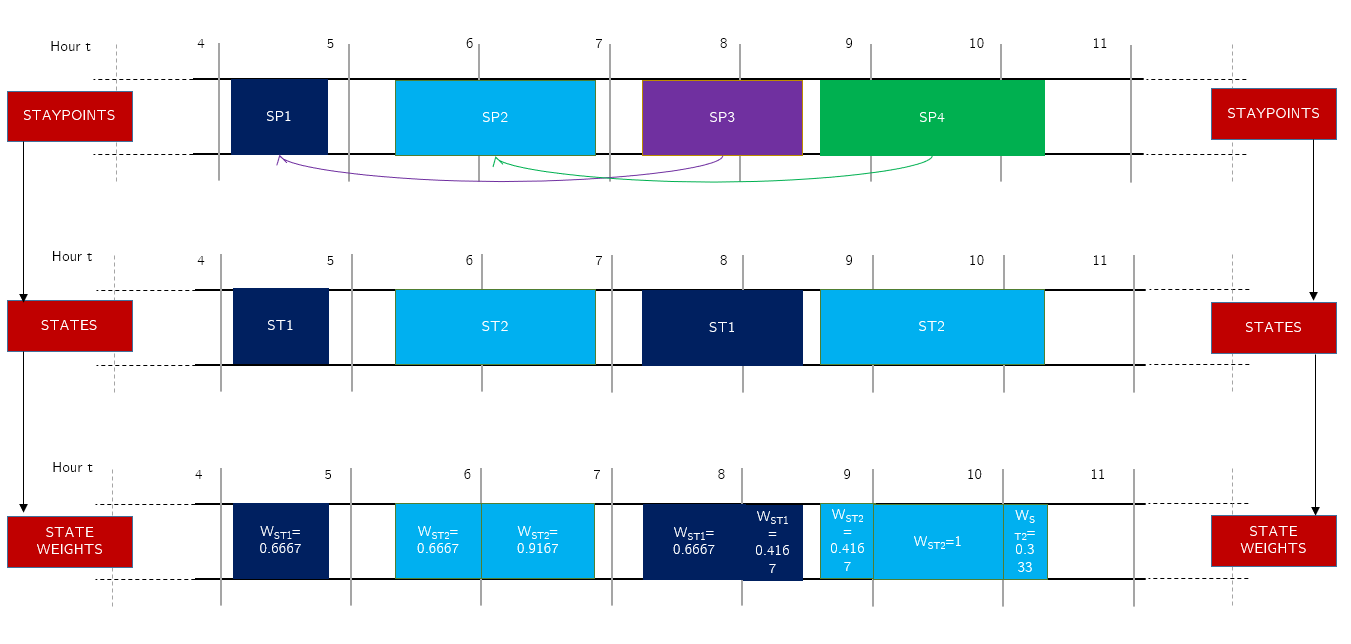
\includegraphics[scale=.54]{threestepsover.png}
\caption{Algorithm Flow-chart}
\label{fig:flow-chart}
\end{figure}

\section{Definitions}
\begin{itemize}
	\item \textbf{Stay-points:} Stay-points are any points which are stayed by the user in user trajectories or it is the start or the end of the trajectory. For example, if user start at his home, the home itself is a stay-point. Now he move towards work, but he visit a cafe in between for breakfast. The cafe is also a stay-point and then he finishes his trajectory at work, where work is again a stay-point. The places like cafe in this case is identified using distance and time based clustering. For example, a set of points within 200m with total duration of stay greater than 20 minutes can be regarded as a stay-point within the trajectory.
	\item \textbf{State:} A state is formed using a group of stay-points. This is done using a distance threshold for states. All the stay-points within this threshold distance are grouped together as a single state. This is called snapping stay-points to the states. The mean of all location latitudes and longitudes from stay-points within a state are stored per state. Finally Markov Chain model is applied to the states. \textit{Note: A new stay-point is only added to the state if after calculating the mean of the new state, all the existing stay-points still stay within the distance threshold from this mean. This is done to avoid drifting problem while aggregating the stay-points into states.}
\end{itemize}

\section{Algorithms}

\begin{algorithm}
\caption{Read new location and process}
\label{pseudoPSO}
\begin{algorithmic}[1]
\For{each newpoint[x, y, d]}
\State $newHour \gets d_h$
\State $newDate \gets d_d$
\If{$newHour != prevHour$}
	\State $prevHour \gets newHour$
	\State calculateLastHourStayPoints()
	\State formStates()
	\State calculateStateLastHourWeights()
	\If{$newDate != prevDate$}
		\State $prevDate \gets newDate$
		\State recalculateMarkovModel()
	\EndIf
\EndIf
\EndFor
\end{algorithmic}
\end{algorithm}

\begin{algorithm}
\caption{calculateLastHourStayPoints() : Calculate last hour stay-points}
\label{pseudoPSO}
\begin{algorithmic}[1]

\For{each  lst\_hr\_pts[x, y, d]}
\If{$d(i) - d(i-1) > th\_tck$}
	\State$ sp \gets lst\_hr\_pts(i),  lst\_hr\_pts(i-1)$
	\State recalculateStartEndStaypoint()
\EndIf

\If{$distance( lst\_hr\_pts(i), cluster) <=   th\_d$}
	\State $cluster \gets add lst\_hr\_pts(i)$ 
	\State calculate Cluster Means
\Else
	\If{$(cluster != empty$) And $duration(cluster) >= th\_t$}
    	\State $sp \gets cluster$
    	\State recalculateStartEndStaypoint()
	\EndIf
\EndIf

\EndFor
\end{algorithmic}
\end{algorithm}

\begin{algorithm}
\caption{recalculateStartEndStaypoint() : Calculte start-end of staypoints}
\label{pseudoPSO}
\begin{algorithmic}[1]
\For{each sp}
	\State $distance \gets distance(sp(i), sp(i+1)$
	\State $time \gets timeDifference(sp(i), sp(i+1)$
	\State $AvgSpeed \gets distance/time$
	\State $AddTime \gets min(distance$, $thresholdDistance)/AvgSpeed$
	\State Update endTime for sp(i)
	\State Update startTime for sp(i+1)
\EndFor
\end{algorithmic}
\end{algorithm}


\begin{algorithm}
\caption{formStates() : Form states from stay-points}
\label{pseudoPSO}
\begin{algorithmic}[1]

\For{each st }
\If{$distance(st(i), st(i+1)) <= th\_d$}
	\State calculate new state mean latitude, mean longitude
	\If{distance(All (orig lat, orig lon) forming st(i) , st(i+1)) $<=$ th\_d}
	\State combine st(i), st(i+1)
	\State calculate combined st Means
	\EndIf
\EndIf
\EndFor
\end{algorithmic}
\end{algorithm}

\begin{algorithm}
\caption{calculateStateLastHourWeights() : Calculate Hourly Weights of States}
\label{pseudoPSO}
\begin{algorithmic}[1]
\State This creates a weights of all states from 0 Hrs to 24 Hrs for each date
\For{each st }

\If{($Hour Changes$) Or ($StateID Changes$)}
	\State $st\_hr\_wt \gets st(i), startTime, endTime$
\EndIf
\EndFor
\end{algorithmic}
\end{algorithm}


\begin{algorithm}
\caption{recalculateMarkovModel() : Recalculate the Markov Model(This algorithm creates the transition probabilities from state i to i+1 from hour j to j+1)}
\label{pseudoPSO}
\begin{algorithmic}[1]
\State 
\For{each $jth-Hour$ from $0to24$ }
	\For{each ith-st}
	\State $mc \gets st\_hr\_wt[i][j] * st\_hr\_wt[i+1][j]$
	\EndFor
\EndFor
\end{algorithmic}
\end{algorithm}

\end{document}



